\documentclass[]{article}

\usepackage[left=2.00cm, right=2.00cm, top=2.00cm, bottom=2.00cm]{geometry}
\usepackage[spanish,es-noshorthands]{babel}
\usepackage[utf8]{inputenc} % para tildes y ñ
\usepackage{graphicx} % para las figuras
\usepackage{xcolor}
\usepackage{listings} % para el código fuente en c++

\lstdefinestyle{customc}{
  belowcaptionskip=1\baselineskip,
  breaklines=true,
  frame=single,
  xleftmargin=\parindent,
  language=C++,
  showstringspaces=false,
  basicstyle=\footnotesize\ttfamily,
  keywordstyle=\bfseries\color{green!40!black},
  commentstyle=\itshape\color{gray!40!gray},
  identifierstyle=\color{black},
  stringstyle=\color{orange},
}
\lstset{style=customc}


%opening
\title{Práctica 1. Algoritmos devoradores}
\author{Miguel Angel Chaves Perez \\ % mantenga las dos barras al final de la línea y este comentario
miguelangel.chavesperez@alum.uca.es \\ % mantenga las dos barras al final de la línea y este comentario
Teléfono: 675287145 \\ % mantenga las dos barras al final de la linea y este comentario
NIF: 49071750p \\ % mantenga las dos barras al final de la línea y este comentario
}


\begin{document}

\maketitle

%\begin{abstract}
%\end{abstract}

% Ejemplo de ecuación a trozos
%
%$f(i,j)=\left\{ 
%  \begin{array}{lcr}
%      i + j & si & i < j \\ % caso 1
%      i + 7 & si & i = 1 \\ % caso 2
%      2 & si & i \geq j     % caso 3
%  \end{array}
%\right.$

\begin{enumerate}
\item Describa a continuación la función diseñada para otorgar un determinado valor a cada una de las celdas del terreno de batalla para el caso del centro de extracción de minerales. 




Se implementas dos estructura de la lista List<AStarNode*> para obtener lista de los nodos abiertos y cerrados:

	. La lista cerrado se guardará nodos visitados y la lista abierto los nodos que aún no ha sido visitados
	. AstarNode* curren para saber que nodo tenemos actualmente
	. current sera expandido y mirara sus hijos para luego introducirlo en la lista abierta
	. al expandir current nos encontramos con un hijo que se encuentra en la lista de abiertos, se comprobara si es o no mejor seguir con ese nodo o repercutir 		hacía el padre
	. Si es mejor se cambiara el nodo actual current por el padre
	. Se suma un valor addicional a cada celda que representa un peso mayor o menor a la defensa principal,todo esto con la ayuda de la matriz additionalCost.







\item Diseñe una función de factibilidad explicita y descríbala a continuación.


Se crea un vector para guardar los distintos valores de las defensas y una matriz donde se almacenaran los valores máximos que se puede obtener dado un numero de defensas y ases.




\item A partir de las funciones definidas en los ejercicios anteriores diseñe un algoritmo voraz que resuelva el problema para el caso del centro de extracción de minerales. Incluya a continuación el código fuente relevante. 

\begin{lstlisting}
void DEF_LIB_EXPORTED placeDefenses(bool** freeCells, int nCellsWidth, int nCellsHeight, float mapWidth, float mapHeight
              , std::list<Object*> obstacles, std::list<Defense*> defenses) 
{

  float cellWidth = mapWidth / nCellsWidth; //Calculamos el ancho de una celda
  float cellHeight = mapHeight / nCellsHeight; //Calculamos el alto de una celda
  float** valorCelda = new float*[nCellsHeight]; // Puntuación para las celdas

  //Inicializamos todas las celdas del mapa con el valor nulo
  for(int i=0; i<nCellsHeight; i++)
  {
    valorCelda[i] = new float[nCellsHeight];
    for(int j=0; j<nCellsHeight; j++)
    valorCelda[i][j] = 0;
  }

  List<Defense*>::iterator currentDefense = defenses.begin();

  //Valores de las celda para la colocacion del centro extrator
  valorCeldaExtratora(valorCelda,cellHeight,obstacles,nCellsWidth);
    
  bool asignada = false;

  //Algorizmo voraz para la colocacion de la celda extractora
  while(!asignada)//mientras que no se haya asignado el valor a la celda extratora
  {
    int coorX,coorY;

    seleccion(valorCelda, &coorX, &coorY,nCellsWidth);//Seleccionamos candidatos
    
    //puntos medios
    float puntoMedioY = coorY*cellHeight + cellHeight/2;
    float puntoMedioX = coorX*cellWidth + cellWidth/2;

    //Comprobacion si es posible esa solucion
    if(factibilidad(puntoMedioX,puntoMedioY,obstacles,defenses,(*currentDefense)->radio,mapWidth))
    {   
      (*currentDefense)->position.x = puntoMedioX;
      (*currentDefense)->position.y = puntoMedioY;
      (*currentDefense)->position.z = 0; 
      asignada = true;
    }
  }
}
\end{lstlisting}


\item Comente las características que lo identifican como perteneciente al esquema de los algoritmos voraces. 

Escriba aquí su respuesta al ejercicio 4.

Conjunto de candidatos: Cada celdas del mapa
Conjunto de candidatos seleccionados: Las celdas con la mayor puntación para la colocación de las defensas
Conjunto de solución: Se comprueba que las defensas y la extractora han sido colocadas y no hay mas candidatos, aunque podría ser no óptima
conjunto de selección: Se comprueba la primera celda que encuentra de menor valor en el terreno, pudiendo o no, ser la solución óptima.
Función de factibilidad: Se comprueba que la defensa o extractor se puede colocar en la celda candidata, si no, se sigue buscando mas candidatos
Función objetivo: Maximizar el tiempo transcurridos sin que los ucos invadan la defensa extractora



\item Describa a continuación la función diseñada para otorgar un determinado valor a cada una de las celdas del terreno de batalla para el caso del resto de defensas. Suponga que el valor otorgado a una celda no puede verse afectado por la colocación de una de estas defensas en el campo de batalla. Dicho de otra forma, no es posible modificar el valor otorgado a una celda una vez que se haya colocado una de estas defensas. Evidentemente, el valor de una celda sí que puede verse afectado por la ubicación del centro de extracción de minerales.

Escriba aquí su respuesta al ejercicio 5.

Determino el valor de cada una de las celdas con su distancia euclídeas a la posición de la defensa extractora. Por lo tanto una puntación menor sera un buen candidato.
Con ello se consigue que la defensa extractora este rodeadas de las demás defensas, y así poder aguantar los ataques de los ucos




\item A partir de las funciones definidas en los ejercicios anteriores diseñe un algoritmo voraz que resuelva el problema global. Este algoritmo puede estar formado por uno o dos algoritmos voraces independientes, ejecutados uno a continuación del otro. Incluya a continuación el código fuente relevante que no haya incluido ya como respuesta al ejercicio 3. 

\begin{figure}[!ht]
\begin{center}
  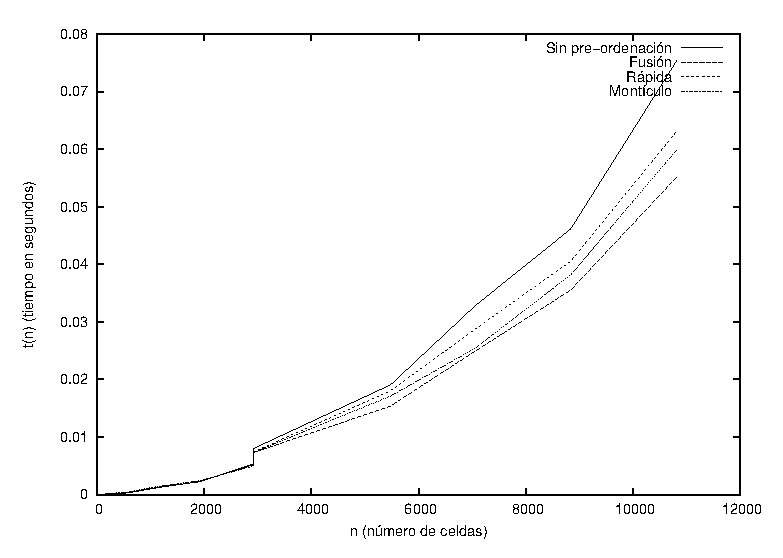
\includegraphics[width=0.9\textwidth]{graphic.eps}
  \caption{Gráfica}
\end{center}
\end{figure} 


\end{enumerate}

Todo el material incluido en esta memoria y en los ficheros asociados es de mi autoría o ha sido facilitado por los profesores de la asignatura. Haciendo entrega de este documento confirmo que he leído la normativa de la asignatura, incluido el punto que respecta al uso de material no original.

\end{document}
